\section{Trace moments for iterated matrix multiplication}
\label{sec:moments}

We now choose the partition of the layers and prove that its mixed operator
has large rank on iterated matrix multiplication.  The parameters remain
those of~\eqref{eq:parameters}.  Arrange the groups along the matrix product
in the order
\begin{equation}
  VU^{\ell_1}\,VU^{\ell_2}\cdots VU^{\ell_k},
  \qquad
  \ell_i=1+\left\lfloor\frac{is}{k}\right\rfloor
             -\left\lfloor\frac{(i-1)s}{k}\right\rfloor.
  \label{eq:balanced-schedule}
\end{equation}
For sufficiently large $n$ we have $0<s/k<1$, so each $\ell_i$ is either
one or two.  Their sum is $k+s=m$.  Thus this word has exactly $k$ layers
in $V$ and $m$ in $U$, and no two $V$ layers are adjacent.  Every layer
contributes all its $n^2$ variables to its group, including the variables
of the first and last matrices that do not occur in the $(1,1)$ entry.

Put $f=\IMM_{n,n}$ and $L=n-1$.  A path $P$ is a sequence
$(p_0,\ldots,p_n)$ with $p_0=p_n=1$ and $p_1,\ldots,p_{n-1}\in[n]$.
Its coordinate in layer $t$ is
\[
  E_t(P)=x^{(t)}_{p_{t-1},p_t}.
\]
There are $n^L$ paths, and $f$ is the sum of the products of their layer
coordinates.  In particular, $f$ has bidegree $(k,m)$, so its finite map
$F_f$ is the restriction of the full operator $T_f=f(\partial_V,U)$ to
$\HH_V(a)\otimes\HH_U(b)$.

\begin{proposition}
\label{prop:imm}
Over $\C$, for the partition~\eqref{eq:balanced-schedule}, there is an
absolute constant $C$ such that, for all sufficiently large $n$,
\[
  R(\IMM_{n,n})\ge D\exp(-C\sqrt n).
\]
\end{proposition}

The proof uses two trace moments.  Give every homogeneous polynomial
space the inner product in which
\[
  \frac{z^M}{\sqrt{M!}},\qquad |M|=t,
  \qquad M!=\prod_i M_i!,
\]
is an orthonormal basis.  This is the finite homogeneous part of the
Bargmann--Fock polynomial normalization~\cite{Bargmann1962}.
Use the tensor product of these inner products
for the domain and codomain of $F_f$, and write
\[
  T=\tr(F_f^*F_f),\qquad
  T_2=\tr\bigl((F_f^*F_f)^2\bigr).
\]
If $T>0$, Cauchy--Schwarz applied to the nonzero eigenvalues of
$F_f^*F_f$ gives
\begin{equation}
  R(f)\ge \frac{T^2}{T_2}.
  \label{eq:trace-rank}
\end{equation}
Define
\[
  A=\frac av,\qquad B=\frac bu,\qquad
  \mu=A^k(1+B)^m.
\]
We will prove the bounds
\[
 T\ge Dn^L\mu\exp(-O(n^{-1/2})),\qquad
 T_2\le Dn^{2L}\mu^2\exp(O(\sqrt n)).
\]
This section reduces
the second bound to a sum over two-letter words; the next section bounds
that sum and completes Proposition~\ref{prop:imm}.

\subsection{Occupation moments}

A uniformly chosen basis vector of $\HH_V(a)\otimes\HH_U(b)$ has two
independent exponent vectors: one is uniform among weak compositions
of $a$ into $v$ parts, and the other among weak compositions of $b$
into $u$ parts.  We compare their moments with those of independent
geometric variables.  For an integer $d\ge0$, write
\[
  (z)_d=z(z-1)\cdots(z-d+1),\qquad
  r^{\overline d}=r(r+1)\cdots(r+d-1),
\]
with both empty products equal to one.

\begin{lemma}
\label{lem:occupation-moments}
Let $M=(M_1,\ldots,M_r)$ be uniform among the weak compositions of an
integer $t\ge0$ into $r\ge1$ parts.  For integers $d_i\ge0$ and
$H=\sum_i d_i$,
\begin{equation}
  \mathbb E\prod_i(M_i)_{d_i}
   =\frac{(t)_H}{r^{\overline H}}\prod_i d_i!.
  \label{eq:composition-moment}
\end{equation}
The right side is zero when $H>t$.

Let $Z_1,\ldots,Z_r$ be independent geometric variables on the
nonnegative integers with mean $G=t/r$.  If a polynomial $P$ has
nonnegative coefficients in the basis
$\{\prod_i(z_i)_{d_i}\}$, then
\begin{equation}
  \mathbb E P(M)\le\mathbb E P(Z).
  \label{eq:occupation-upper}
\end{equation}
If $t>0$ and all terms of that expansion have total order at most
$H_0\le t/2$, then also
\begin{equation}
  \mathbb E P(M)
  \ge
  \exp\left(-\frac{H_0^2}{t}-\frac{H_0^2}{2r}\right)
  \mathbb E P(Z).
  \label{eq:occupation-lower}
\end{equation}
\end{lemma}

\begin{proof}
For $d\ge0$,
\[
  \sum_{j\ge0}(j)_d y^j=\frac{d!y^d}{(1-y)^{d+1}}.
\]
If $H\le t$, coefficient extraction therefore gives
\[
  \sum_{|M|=t}\prod_i(M_i)_{d_i}
    =\left(\prod_i d_i!\right)
       \binom{t+r-1}{t-H}.
\]
Divide by $\binom{t+r-1}{t}$ to obtain
\eqref{eq:composition-moment}.  If $H>t$, every composition has
$M_i<d_i$ for some $i$, so every summand is zero, as is $(t)_H$.

For $G>0$, the geometric law is
\[
  \Pr(Z_i=j)=\frac1{1+G}\left(\frac{G}{1+G}\right)^j
  \quad(j\ge0),
\]
and its factorial moment is $\mathbb E(Z_i)_d=d!G^d$.  For $H\le t$
the ratio of the moment in~\eqref{eq:composition-moment} to the
corresponding independent geometric moment is
\begin{equation}
  \prod_{j=0}^{H-1}\frac{1-j/t}{1+j/r}.
  \label{eq:occupation-ratio}
\end{equation}
It is at most one.  For $H>t$ the composition moment is zero, so the
same upper comparison holds.  When $H\le H_0\le t/2$, the inequalities
$\log(1-x)\ge-2x$ for $0\le x\le1/2$ and
$\log(1+x)\le x$ for $x\ge0$ show that the logarithm of
\eqref{eq:occupation-ratio} is at least
\[
  -\sum_{j=0}^{H-1}\left(\frac{2j}{t}+\frac{j}{r}\right)
  \ge -\frac{H_0^2}{t}-\frac{H_0^2}{2r}.
\]
Sum these comparisons with the nonnegative coefficients of $P$.
If $t=0$, both $M$ and the geometric vector of mean zero are identically
zero, giving~\eqref{eq:occupation-upper} directly.
\end{proof}

The comparison is termwise and does not assert independence of the
coordinates of $M$.  We apply it separately in the two groups.
By Lemma~\ref{lem:parameters}, total orders at most $2n$ satisfy the
lower-bound hypothesis, and their combined logarithmic loss is
\begin{equation}
  O\left(\frac{n^2}{a}+\frac{n^2}{v}
          +\frac{n^2}{b}+\frac{n^2}{u}\right)
  =O(n^{-1/2}).
  \label{eq:occupation-loss}
\end{equation}

\subsection{The first trace}

In the chosen orthonormal bases, differentiation and multiplication
act by
\[
  \partial_i\frac{z^M}{\sqrt{M!}}
    =\sqrt{M_i}\frac{z^{M-\mathbf e_i}}{\sqrt{(M-\mathbf e_i)!}},
  \qquad
  z_i\frac{z^M}{\sqrt{M!}}
    =\sqrt{M_i+1}\frac{z^{M+\mathbf e_i}}{\sqrt{(M+\mathbf e_i)!}}.
\]
The derivative is zero when $M_i=0$; its displayed expression is used
only when $M_i\ge1$.  Here $\mathbf e_i$ is the coordinate unit vector.
In particular, repeated differentiation of order $d$ has coefficient
$\sqrt{(M_i)_d}$, with no additional factorial divisor.

Index a domain basis vector by the combined exponent vector $M$ on
$V\cup U$, with totals $a$ and $b$ in the two groups.  The summand of
$F_f$ corresponding to a path $P$ shifts this vector by
\[
  \epsilon_P
  =-\sum_{t:\,V}\mathbf e_{E_t(P)}
    +\sum_{t:\,U}\mathbf e_{E_t(P)}
\]
with coefficient
\begin{equation}
  c_P(M)
    =\left(
       \prod_{t:\,V}M_{E_t(P)}
       \prod_{t:\,U}(M_{E_t(P)}+1)
      \right)^{1/2}.
  \label{eq:path-coefficient}
\end{equation}
A shift requiring a negative occupation contributes zero.  We extend
the coefficient notation by zero to invalid input indices as well.
Different layers have disjoint coordinates, so a path never repeats a
coordinate.  Moreover, the shifts $\epsilon_P$ are distinct: a shift
specifies the coordinate in every layer and hence every vertex of $P$.

Consequently different paths from the same input reach different
output indices.  Summing the squared entries of $F_f$ gives the exact
identity
\[
  T=D\sum_P\mathbb E\left[
       \prod_{t:\,V}M_{E_t(P)}
       \prod_{t:\,U}(M_{E_t(P)}+1)
      \right],
\]
where the expectation is over the uniform domain indices.  Every
polynomial inside this expectation has nonnegative falling-factorial
coefficients.  Under independent geometric occupations of means $A$
and $B$, its expectation is $\mu$.  Lemma~\ref{lem:occupation-moments}
and~\eqref{eq:occupation-loss} therefore imply
\begin{equation}
  T\ge Dn^L\mu\exp(-O(n^{-1/2}))>0.
  \label{eq:first-trace}
\end{equation}
The inactive endpoint coordinates are included in the uniform
compositions and in $v,u$ throughout; they introduce no additional
factor into this calculation.

\subsection{Four paths in the second trace}

The matrix entries of $F_f$ in these bases are real and nonnegative.
An entry of $F_f^*F_f$ indexed by $M,M'$ is the sum of
$c_P(M)c_Q(M')$ over pairs of paths satisfying
$M+\epsilon_P=M'+\epsilon_Q$.  Squaring its entries and summing yields
\begin{equation}
\begin{split}
  T_2
   &=D\,\mathbb E_M
      \sum_{\substack{P,Q,R,S:\
        \epsilon_P-\epsilon_Q=\epsilon_R-\epsilon_S}}
        c_P(M)c_Q(M')c_R(M)c_S(M'),\\[-2pt]
  &\hspace{34mm} M'=M+\epsilon_P-\epsilon_Q.
\end{split}
  \label{eq:four-path-trace}
\end{equation}
The zero convention handles invalid indices.  There is no additional
sum over $M'$, because $M,P,Q$ determine it.

The condition on four paths holds separately in each layer.  Denoting
their four coordinates in that layer by $p,q,r,s$, respectively, it is
$\mathbf e_p-\mathbf e_q=\mathbf e_r-\mathbf e_s$.  If this difference
is zero, then $p=q$ and $r=s$.  Otherwise its positive and negative
coordinates force $p=r$ and $q=s$, with $p\ne q$.  Thus there are exactly
two types:
\[
\begin{array}{c|l}
  \mathcal N & p=q=i,\quad r=s=j,\\
  \mathcal D & p=r=i,\quad q=s=j,\quad i\ne j.
\end{array}
\]
The all-equal case belongs to $\mathcal N$.  For each compatible
quadruple, the four-coefficient product in~\eqref{eq:four-path-trace}
is a product over layers of the following polynomials:
\begin{equation}
\begin{array}{c|cc}
  &\mathcal N&\mathcal D\\ \hline
  V&M_iM_j&M_i(M_j+1)\\
  U&(M_i+1)(M_j+1)&(M_i+1)M_j.
\end{array}
  \label{eq:local-polynomials}
\end{equation}
Indeed, the shift from $M$ to $M'$ is zero in type $\mathcal N$.
In a $V$ layer of type $\mathcal D$ it is $-\mathbf e_i+\mathbf e_j$,
so the two coefficients at $M$ contribute $M_i$ and the two at $M'$
contribute $M_j+1$.  In a $U$ layer of type $\mathcal D$ the shift is
$\mathbf e_i-\mathbf e_j$, giving $(M_i+1)M_j$ instead.

These polynomial formulas also account for invalid indices.  In type
$\mathcal D$, a negative coordinate of $M'$ requires $M_i=0$ in a $V$
layer or $M_j=0$ in a $U$ layer, and the corresponding table entry
vanishes.  In type $\mathcal N$, an unavailable derivative makes
$M_iM_j$ zero.  Since different layers use distinct coordinates, these
exhaust the possible failures.  Thus the product in
\eqref{eq:local-polynomials} equals the zero-extended contribution.

When $i=j$ in type $\mathcal N$, the required expansions are
\[
  z^2=(z)_2+(z)_1,
  \qquad
  (z+1)^2=(z)_2+3(z)_1+1.
\]
All other table entries are products of $(z)_1$ and $(z)_1+1$ on distinct
coordinates.  Hence every product of local entries has nonnegative
falling-factorial coefficients, with order at most $2k$ in $V$ and
$2m$ in $U$.  Lemma~\ref{lem:occupation-moments} bounds its expectation
by the expectation for independent geometric occupations.

For a geometric variable $Z$ of mean $G$,
$\mathbb EZ^2=2G^2+G$ and
$\mathbb E(Z+1)^2=2G^2+3G+1$.  Dividing the geometric expectations in
each $V$ layer by $A^2$ and in each $U$ layer by $(1+B)^2$, we obtain
\begin{equation}
\begin{array}{c|cc}
  &\mathcal N&\mathcal D\\ \hline
  V&1+\alpha^{-1}\mathbf1_{\{i=j\}}&\alpha^{-1}\\
  U&1+\beta\mathbf1_{\{i=j\}}&\beta.
\end{array}
  \label{eq:local-weights}
\end{equation}
Here $(A+1)/A=\alpha^{-1}$ and $B/(B+1)=\beta$.  For example,
the repeated-coordinate $V$ entry is
$(2A^2+A)/A^2=1+\alpha^{-1}$, so the repeated factorial contribution
has been retained.  The product of the normalizing factors over all
layers is $\mu^2$.

\subsection{A sum over pairing types}

Assign to a compatible quadruple its type word
$\tau\in\{\mathcal N,\mathcal D\}^n$.  For each such word, enlarge its
class of quadruples by dropping the inequalities $i\ne j$ at all
$\mathcal D$ layers.  Keep their weights equal to $\alpha^{-1}$ and
$\beta$ as in~\eqref{eq:local-weights}.  These are assigned weights on
the newly admitted tuples, not their geometric occupation moments.
Every original tuple retains its weight, and every new weight is
nonnegative, so this enlargement gives an upper bound.

Equality of matrix-entry coordinates equates the path labels at both
ends of that layer.  The relaxed equalities can therefore be counted
independently at every internal vertex.  A layer of type $\mathcal N$
pairs the paths as
$\{P,Q\},\{R,S\}$, while a layer of type $\mathcal D$ pairs them as
$\{P,R\},\{Q,S\}$.  At a vertex between layers of the same type, there
are two free labels in $[n]$.  At a vertex between different types the
two pairings together identify all four labels, leaving one free label.
These give $n^2$ and $n$ choices, respectively, as illustrated in
Figure~\ref{fig:pairings}.
The two external vertex labels are fixed to $1$.  Every independent
choice at the internal vertices gives four paths, because all matrix
entries are available, and every relaxed quadruple arises uniquely
this way.  The set of assignments is therefore a Cartesian product
over internal vertices.  If
\[
  w(\tau)=\#\{t\in\{1,\ldots,n-1\}:\tau_t\ne\tau_{t+1}\},
\]
the number of assignments is exactly $n^{2L-w(\tau)}$.

\begin{figure}[tbp]
\centering
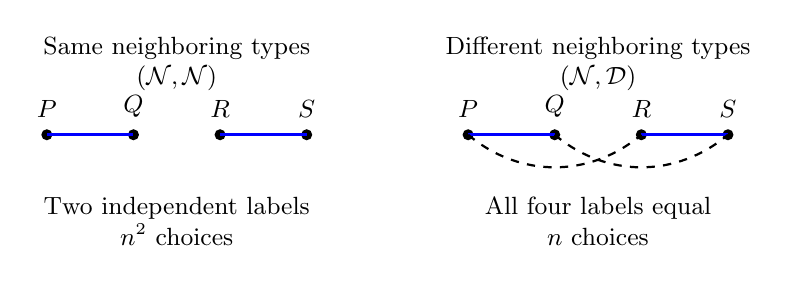
\begin{tikzpicture}[x=1cm,y=1cm,every node/.style={font=\small}]
  \node[align=center] at (1.65,1.65) {Same neighboring types\\($\mathcal N,\mathcal N$)};
  \node[align=center] at (7.0,1.65) {Different neighboring types\\($\mathcal N,\mathcal D$)};
  \foreach \x/\name in {0/P,1.1/Q,2.2/R,3.3/S,5.35/P,6.45/Q,7.55/R,8.65/S} {
    \fill (\x,0.75) circle (2pt);
    \node[above] at (\x,0.85) {$\name$};
  }
  \draw[very thick,blue] (0,0.75) -- (1.1,0.75);
  \draw[very thick,blue] (2.2,0.75) -- (3.3,0.75);
  \draw[very thick,blue] (5.35,0.75) -- (6.45,0.75);
  \draw[very thick,blue] (7.55,0.75) -- (8.65,0.75);
  \draw[thick,dashed] (5.35,0.75) to[bend right=40] (7.55,0.75);
  \draw[thick,dashed] (6.45,0.75) to[bend right=40] (8.65,0.75);
  \node[align=center] at (1.65,-0.35) {Two independent labels\\$n^2$ choices};
  \node[align=center] at (7.0,-0.35) {All four labels equal\\$n$ choices};
\end{tikzpicture}
\caption{Equality constraints on the four path labels at one internal
vertex after the $\mathcal D$ inequalities are relaxed.  Type $\mathcal N$ pairs $P,Q$
and $R,S$ (solid edges); type $\mathcal D$ pairs $P,R$ and $Q,S$ (dashed edges).
Equal neighboring types leave two free labels.  A change of type
identifies all four, contributing a factor $n^{-1}$ to the count.
The same two-label count holds for neighboring types $\mathcal D,\mathcal D$.}
\label{fig:pairings}
\end{figure}


For a layer $t$ of type $\mathcal N$, let $h_t$ be the number of its
end vertices that are internal and lie between two layers of type
$\mathcal N$.  At each of these vertices the two free labels are
independent and uniform in $[n]$, so they agree with probability $1/n$.
At an external vertex or an interface between different types the
labels already agree.  Consequently the two coordinates $i,j$ of
this $\mathcal N$ layer agree with probability $n^{-h_t}$.

The end-vertex sets of different $V$ layers are disjoint, because no
two $V$ layers are adjacent in~\eqref{eq:balanced-schedule}.  Under
the uniform distribution on the Cartesian product of relaxed vertex
assignments, the equality events just described are therefore
independent for the $\mathcal N$ layers in $V$.  Their average weight
is
\[
  \prod_{t:\,\tau_t=\mathcal N,\ t\text{ in }V}
       (1+\alpha^{-1}n^{-h_t}).
\]
For each $\mathcal N$ layer in $U$ we instead bound its weight
pointwise by $1+\beta$, so no independence assertion for these layers
is needed.

Write $d_V(\tau)$ and $d_U(\tau)$ for the numbers of $\mathcal D$
layers in $V$ and $U$, respectively, and put
$N_V(\tau)=\{t:t\text{ is in }V,\ \tau_t=\mathcal N\}$.
Combining the occupation comparison, the relaxed assignment count,
and the preceding weight estimates proves
\begin{equation}
  \frac{T_2}{Dn^{2L}\mu^2}
  \le (1+\beta)^m
       \sum_{\tau\in\{\mathcal N,\mathcal D\}^n}
         n^{-w(\tau)}\alpha^{-d_V(\tau)}\beta^{d_U(\tau)}
         \prod_{t\in N_V(\tau)}
             (1+\alpha^{-1}n^{-h_t}).
  \label{eq:moment-reduction}
\end{equation}
Since $\beta\le2/\sqrt n$, the factor $(1+\beta)^m$ is
$\exp(O(\sqrt n))$.  It remains to prove the same bound for the word
sum in~\eqref{eq:moment-reduction}.  Lemma~\ref{lem:word-sum} establishes
this using the spacing of the $V$ layers and the balanced schedule.
